\section{External Interfaces}
\begin{figure}[h]
    \centering
    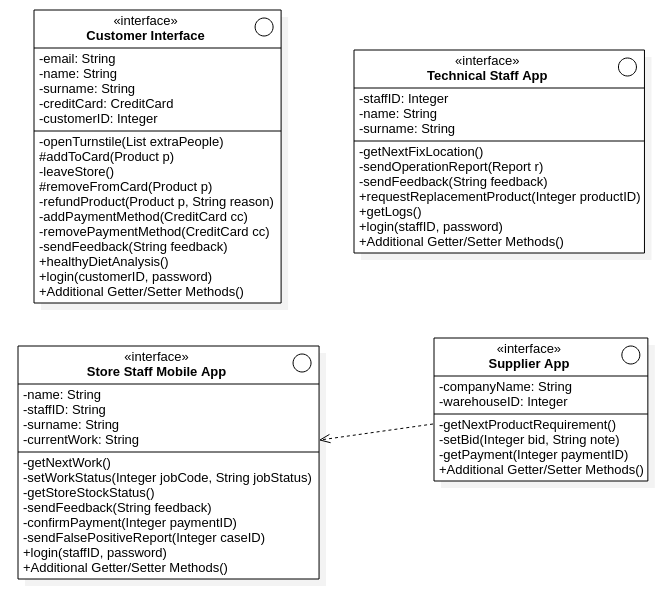
\includegraphics[width=0.9\linewidth]{content/specificRequirements/img/external_interfaces.PNG}
    \caption{External Interface Class Diagram}
    \label{fig:external_interface_class_diagram}
\end{figure}

External interfaces are depicted in \ref{fig:external_interface_class_diagram} diagram where some of them requires additional explanations. The requirements of each part and their detailed description are given below. Note that some of the operations are protected which is because they need to be accessed by inheriting classes which are the guests of a registered customer.

\subsection{Customer Interface}
Customer interface is the interface that the customer will be using. It provides various functions for the customer. Most of them are basic level purchasing functions. The requirements for this interface are :


\begin{itemize}
    \item Email and customer ID shall be unique.
    \item Suspicious and dangerous customers shall not enter to the store.
    \item Removing and adding a product from card should be instant, i.e. in 20 seconds after putting back.
    \item Add payment operation should validate that the card is valid.
    \item Remove payment method should completely remove the card without any residual information
\end{itemize}


\subsection{Technical Staff App}
Technical staff uses app to get the jobs and broken equipment that they need to fix. The staff is also responsible for procuring the broken or needed parts.

\begin{itemize}
    \item Staff ID shall be unique.
    \item Get next fix location should be implemented as a priority queue.
    \item Problems should be fixed based on their importance.
    \item Technical staff feedback should be evaluated regularly, at least once a week.
\end{itemize}


\subsection{Supplier App}
Supplier app is used buy suppliers to bid and supply the required products. Supplier app depends on the store staff mobile app because demand is created by the store staff which then is satisfied. Store staffs are also responsible to confirm the products that are seen to be purchased by the customers, but not purchased in the real scenario where decision making algorithms fail. Store staff uses false positive report system for this purpose.Also, confirmation of supplier product purchases are done by the store staff. The list of requirements are :

\begin{itemize}
    \item Warehouse ID shall be unique.
    \item Different companies shall bid to the same product.
    \item Only one warehouse of a company should be able to bid to auction.
    \item Next product requirements should be implemented as a priority queue.
    \item Payment transfer should be fast, within 2 work days from the product is supplied.
\end{itemize}


\subsection{Store Staff Mobile App}
Store staff uses the app to locate an issue, solve store problems, replace products whose amount is reduces, and report issues in the store. The requirements are :

\begin{itemize}
    \item Staff ID shall be unique.
    \item Only a single work should be assigned a staff at a time.
    \item Works should be implemented as priority queues.
    \item Payments should be confirmed just after a transaction is done.
    \item False positive reports shall be immediate. Any lag in this process has a potential to loss of data about the frauds.
    \item Current work status set should always follow work assignment or store stock query that results in lack of products in the store.
\end{itemize}

